\section{Plugin模块分析}

Plugin用于管理一个或者多个DataMover,其提供一种通用的DataMover操作接口,具体的接口的实现则由用户根据不同的存储后端实现不同的DataMover。Plugin模块的主要架构如下: 

\begin{figure}[!htb]
    \centering
    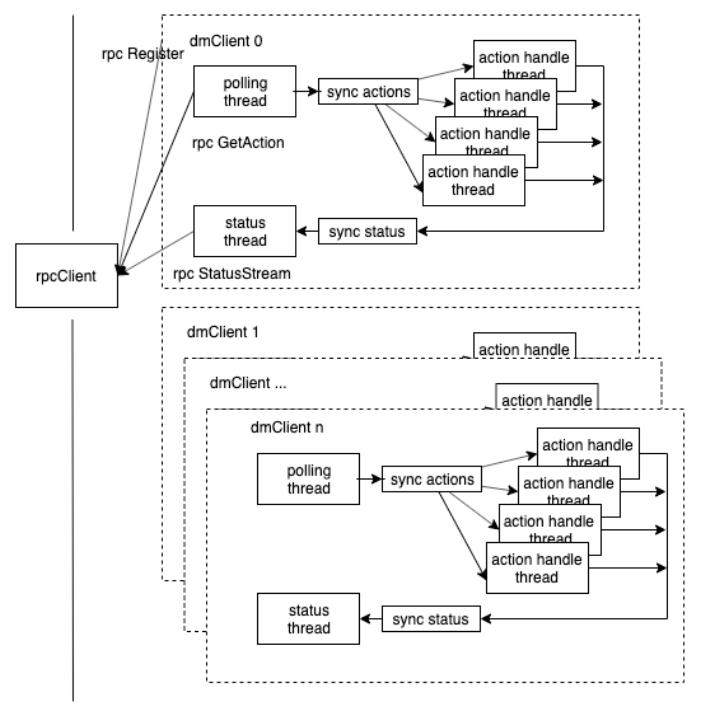
\includegraphics[width=\linewidth]{plugin.png}
    \caption{Plugin模块}\label{fig:region-image}
\end{figure}

Plugin模块定义可一种通用的DataMover操作框架,用户仅需要实现Plugin中定义的archive,restore以及remove操作。在Plugin中,每一个DataMover对应一个dmClient。每个dmClient对应一个archive ID,负责从Proxy中获取属于自己的HSM命令。dmClient在启动时会创建一个polling线程,该线程不断的调用GetAction从Proxy获取一个HSM命令,之后将该命令放到一个同步的全局actions channel中。dmClient启动一个或者多个action handle线程,每个线程从全局的同步channel中不断的读取HSM命令。读取到HSM命令时将调用dmio定义的接口进行数据拷贝,同时该线程不断的将数据拷贝的进度发送到一个同步的全局status channel中。status线程不断的从status channel获取进度数据,并通过调用StatusStream将进度数据不断的发送到Proxy中。 


